\begin{table}[htbp]
	\centering
	\begin{tabular}{|l|l|}
		\hline
		\textbf{Description} & \textbf{Results} \\ \hline
		Timespan & 1964:2021 \\ \hline
		Sources (Journals, Books, etc) & 595 \\ \hline
		Annual Growth Rate \% & 8.94 \\ \hline
		Document Average Age & 8.99 \\ \hline
		Average citations per doc & 5.232 \\ \hline
		References & 43944 \\ \hline
		Documents & 1211 \\ \hline
		- article & 826 \\ \hline
		- book & 18 \\ \hline
		- book chapter & 143 \\ \hline
		- conference paper & 13 \\ \hline
		- editorial & 21 \\ \hline
		- letter & 2 \\ \hline
		- note & 16 \\ \hline
		- review & 171 \\ \hline
		- short survey & 1 \\ \hline
	\end{tabular}
	\caption{Resumen de los datos recolectados}
	\label{tb:resumen}
\end{table}




\begin{figure}[ht]

\centering
\begin{subfigure}[b]{0.48\textwidth}
\centering
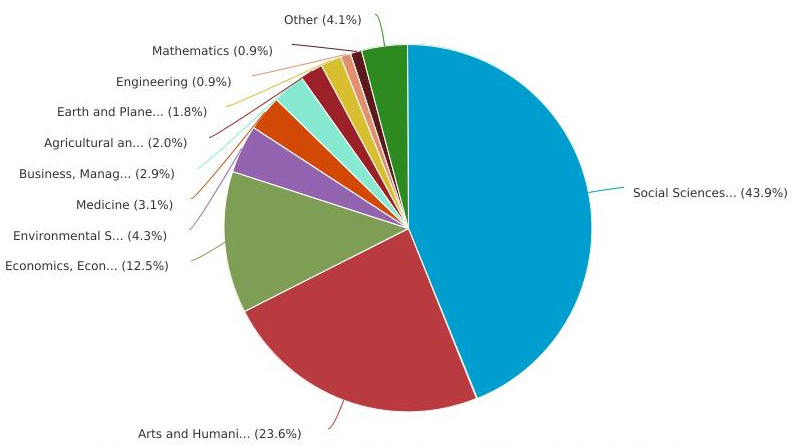
\includegraphics[width=1.1\textwidth]{imagenes/Scopus-Analyze-Subject.jpg}
\caption{Documentos por área de investigación}
\label{fig:docs_area}   
\end{subfigure}
\hfill
\begin{subfigure}[b]{0.48\textwidth}
\centering
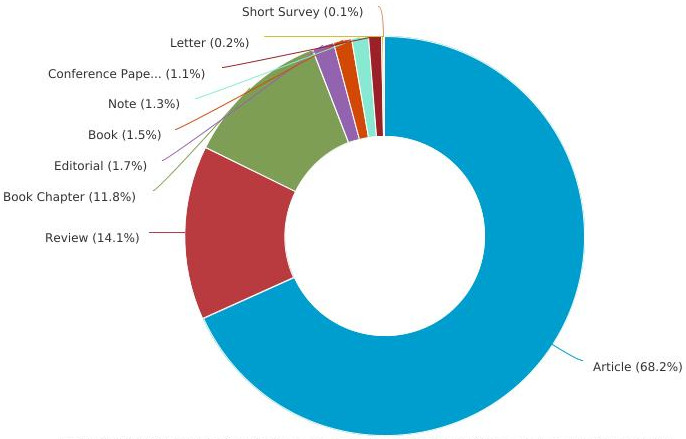
\includegraphics[width=0.95\textwidth]{imagenes/Scopus-Analyze-Doctype.jpg}
\caption{Documentos por tipo.}
\label{fig:docs_tipo} 
\end{subfigure}
\caption{Clasificación de los documentos analizados.}
\label{fig:docs_clasificacion} 
\end{figure}

\begin{figure}[ht]
	
	\centering
	\begin{subfigure}[b]{0.48\textwidth}
		\centering
		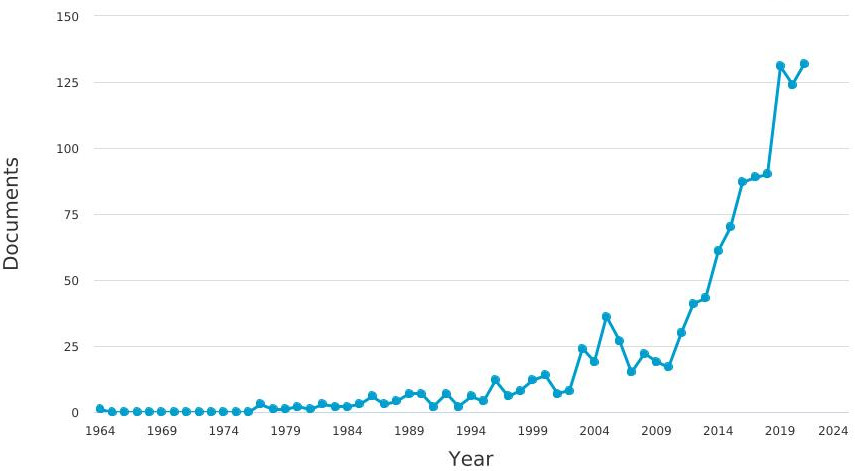
\includegraphics[width=1\textwidth]{imagenes/Scopus-Analyze-Year.jpg}
		\caption{Documentos publicados por año.}
		\label{fig:papers} 
	\end{subfigure}
	\hfill
	\begin{subfigure}[b]{0.48\textwidth}
		\centering
		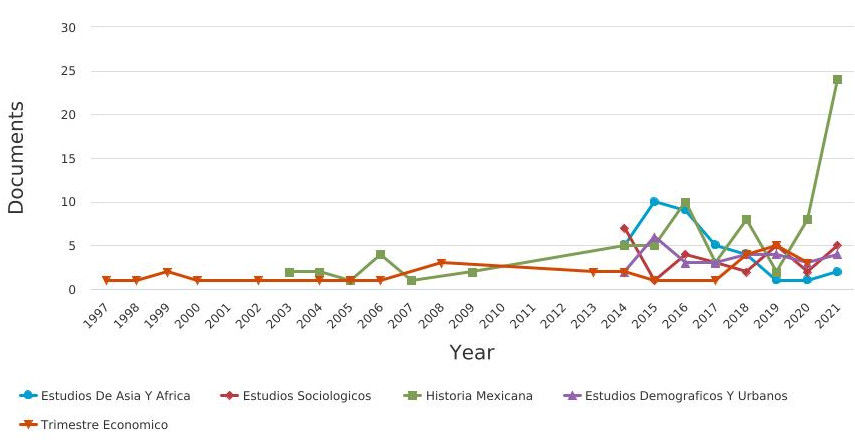
\includegraphics[width=1\textwidth]{imagenes/Scopus-Analyze-Source.jpg}
		\caption{Documentos publicados por año en las 5 fuentes más pupulares.}
		\label{fig:papers} 
	\end{subfigure}
	\caption{Evolución anual de las publicaciones.}
	\label{fig:docs_evolución} 
\end{figure}